\documentclass{beamer}

\usepackage[T1]{fontenc}
\usepackage{inputenc}

\usepackage{amsmath}
\usepackage{listings}
\lstset{
  basicstyle=\footnotesize,
  language=Caml,
  showstringspaces=false,
}


\usetheme{Boadilla}
\usecolortheme{dolphin}
\useoutertheme{infolines}


\setbeamertemplate{footline}
{
  \leavevmode%
  \hbox{%
  \begin{beamercolorbox}[wd=.333333\paperwidth,ht=2.25ex,dp=1ex,center]{author in head/foot}%
    \usebeamerfont{author in head/foot}\insertshortauthor%~~\beamer@ifempty{\insertshortinstitute}{}{(\insertshortinstitute)}
  \end{beamercolorbox}%
  \begin{beamercolorbox}[wd=.333333\paperwidth,ht=2.25ex,dp=1ex,center]{title in head/foot}%
    \usebeamerfont{title in head/foot}\insertshorttitle
  \end{beamercolorbox}%
  \begin{beamercolorbox}[wd=.333333\paperwidth,ht=2.25ex,dp=1ex,right]{date in head/foot}%
    \usebeamerfont{date in head/foot}\insertshortdate{}\hspace*{2em}
    \insertframenumber{} / \inserttotalframenumber\hspace*{2ex}
  \end{beamercolorbox}}%
  \vskip0pt%
}

\title[Sota on attack models and technologies]{State-of-the-art on attack models and technologies}
\author{Maxime Puys}
\date{\today}

\graphicspath{{assets/}}

\begin{document}

\begin{frame}
    \maketitle
\end{frame}

%\begin{frame}
%    \frametitle{Smart Grid}
%
%    \begin{itemize}
%        \item Next generation power supply.
%            \vfill
%        \item Integrates power supply network (e.g.: power lines),
%            \vfill
%        \item {\bf AND} network communications between parts of the system.
%    \end{itemize}
%    \vfill
%    \begin{figure}[htb]
%        \centering
%        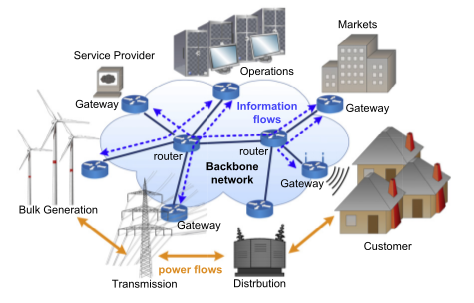
\includegraphics[scale=.6]{smart-grid}
%    \end{figure}
%\end{frame}

\begin{frame}
    \frametitle{Two ways of thinking}

    \begin{block}{Attacks on the SCADA network}
        The ARAMIS module has to avoid attacks comming from one side of the network and targeting the other.
    \end{block}
    \vfill
    \begin{block}{Attacks targeting the module itself}
        The module CAN BE the target of the attack as it shall be the single point of passage.
    \end{block}
\end{frame}

\begin{frame}
    \frametitle{Joint work with safety}

    The documents proposed by ANSSI tell that:
    \vfill
    \begin{itemize}
        \item Most industries focus on safety ({\em s\^uret\'e de fonctionnement})
            \vfill
        \item However ANSSI emphasizes the need of IT security in industry
            \vfill
        \item One can distinguish three types of attacks on industries (targeted, challenges, not targeted)
            \vfill
        \item The concept of {\bf Defense in depth} is realy pushed forward
            \vfill
        \item IT security should be taken into account within the AMDEC or HAZOP analysis methods (which are designed for safety)
    \end{itemize}
\end{frame}

\begin{frame}
    \frametitle{Security requirements}

    Authors analysed security requirements for most SCADA systems:
    \vfill
    \begin{itemize}
        \item {\bf Availability}
        \vfill
        \item {\bf Integrity}
        \vfill
        \item Confidentiality
    \end{itemize}
    \vfill
    \begin{figure}[htb]
        \centering
        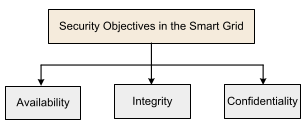
\includegraphics[scale=.6]{objectives}
    \end{figure}
\end{frame}



\section{Availability}

\begin{frame}
    \tableofcontents
\end{frame}

\begin{frame}
    \frametitle{Definition}

    \begin{block}{Availability}
        Ensuring timely and reliable access to and use of information.\\
        \medskip
        {\bf Note:} Importance of time-criticity in communications (e.g.: legacy serial modbus).
    \end{block}
    \vfill
    \begin{block}{Risk}
        Disruption of access to or use of information can have dire consequenses such as an electricity blackout or even cause severe damages to infrastructures.\\
        \medskip
        {\bf Note:} Shall the ARAMIS module block packets or just raise alerts?\\$\rightarrow$ Bypass mode?
    \end{block}
\end{frame}

\begin{frame}
    \frametitle{Attacks on }

    \begin{block}{Denial Of Service}
        Attempt to delay or block communication between entities.
    \end{block}
    \vfill
    Several layers can be attacked:
    \begin{itemize}
        \item Physical layer,
        \item MAC layer,
        \item Network and transport layer,
        \item Application layer.
    \end{itemize}
    \vfill
    {\bf Note:} An adversary does not always need to completly shutdown the trafic but can just delay time-critical messages.
\end{frame}

\begin{frame}
    \frametitle{Physical layer}

    \begin{block}{Channel jamming}
        {\em Brouillage de signal}$_{fr}$ -- Specialy for wireless communications (possible on ethernet using magnetic coils?).\\
        \medskip
        Mostly happens in local area networks due to range limitations.
    \end{block}
\end{frame}

\begin{frame}
    \frametitle{MAC layer}

    \begin{block}{Compromized backoff parameters}
        An adversary (such as a compromized device) can modify at MAC level parameters (such as Clear Channel Assessment threshold or other parameters in CSMA/CA protocols).\\
        \medskip
        This might cause the medium to ignore other users.
    \end{block}
    \vfill
    \begin{block}{MAC spoofing}
        Address mascarading can help sending fake informations to other devices (e.g.: forged packets) through misconfigured access lists.
    \end{block}
\end{frame}

\begin{frame}
    \frametitle{Network and transport layer}

    \begin{block}{Trafic flooding}
        ICMP flood, SYN flood, teardrops attacks.\\
        \medskip
        Software configurations are usualy easily fixed but as SCADA involves quite some legacy devices, it can be a concern.
    \end{block}
    \vfill
    \begin{block}{SCADA example}
        A recent study investigated the impact of a {\bf buffer-flooding attack} on a {\bf DNP3-based SCADA network} with real SCADA system hardware and software, and showed that current SCADA system is quite vulnerable to the DoS attack.

        \begin{figure}[htb]
            \centering
            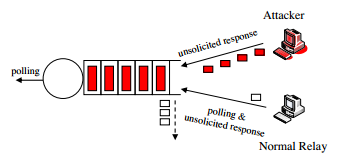
\includegraphics[scale=.35]{dnp3}
        \end{figure}
    \end{block}
\end{frame}

\begin{frame}
    \frametitle{Application layer}

    \begin{block}{Attacks}
        Rather than focus on transmission bandwidth, such attacks intend to exhaust ressources of a computer.\\
        \medskip
        Exploit programming mistakes in programs such as for example network servers (buffer overflows, heap overflows, memory leaks, ...).\\
        \medskip
        {\bf Note:} Complexity attacks.
    \end{block}
\end{frame}

\begin{frame}
    \frametitle{Counter-measures}

    \begin{block}{Detection}
        Measuring the Received Signal Strength Information (RSSI) can detect jamming attacks.\\
        Packet based detections can be performed at every layer to measure a significant increase of packet transmission failures.\\
        \medskip
        Lot of dedicated softwares (such as {\bf netstat}).
    \end{block}
    \vfill
    \begin{block}{Mitigation}
        Rate limiting policies in routers.\\
        Packets filtering (e.g.: firewalls).\\
        \medskip
        (Does not seems to be applicable to ARAMIS) {\bf Network reconfiguration:} Modify the network topology in order to either add more ressources to the victime or to isolate the attack source.
    \end{block}
\end{frame}

\section{Integrity}

\begin{frame}
    \tableofcontents[currentsection]
\end{frame}

\begin{frame}
    \frametitle{Definition}

    \begin{block}{Integrity}
         Maintaining and assuring the accuracy and consistency of data over its entire life-cycle.
    \end{block}
    \vfill
    \begin{block}{Risk}
        A loss of integrity (unauthorized modification or destruction of information) can induce incorrect decision regarding machines.
    \end{block}
\end{frame}

\begin{frame}
    \frametitle{Attacks on }

    \begin{block}{Integrity}
        Either {\bf modifying existant information}\\
        \medskip
        Or {\bf inject new forged information}.
    \end{block}
    \vfill
    Both are called {\bf false data injection}.
    \vfill
    {\bf Objective:} Most of time, impact the state estimation and induce operators into making bad decisions.
    \vfill
    For example: In the case of Smart Grid, such attack could be use to impact the electric market and cause potential financial losses.
\end{frame}

\begin{frame}
    \frametitle{Counter-measures}

    \begin{block}{Detection}
        Cryptographic signatures.\\
        \medskip
        Depending on the hardware, potential efficiency problems (regarding to {\bf availability} property).
        HMAC or PKI signatures -> Key management.
    \end{block}
    \vfill
    \begin{block}{Mitigation}
        Error-correcting codes. Adds redundancy in order to retreive corrupted information.
    \end{block}
\end{frame}

\section{Confidentiality}

\begin{frame}
    \tableofcontents[currentsection]
\end{frame}

\begin{frame}
    \frametitle{Definition}

    \begin{block}{Confidentiality}
         Preserving authorized restrictions on information access and disclosure, mainly to protect personal privacy and proprietary information.
    \end{block}
    \vfill
    \begin{block}{Risk}
        Often said less critical than {\bf availability} and {\bf integrity}.\\
        \medskip
        Becomes crucial when dealing with customers data, credentials or cryptographic keys.
    \end{block}
\end{frame}

\begin{frame}
    \frametitle{Attacks on }

    \begin{block}{Wiretapping}
        {\em \'Ecoutes}$_{fr}$ -- Access to packets contents.
    \end{block}
    \vfill
    \begin{block}{Trafic analyzing}
        Only network topology and flows but not packets contents.
    \end{block}
\end{frame}

\begin{frame}
    \frametitle{Counter-measures}

    \begin{block}{Detection}
        ??? -- To my knowledge, it is not possible to detect a sniffer on a network not using any secure protocol.\\
        If yes, how router would be handle ?
    \end{block}
    \vfill
    \begin{block}{Mitigation}
        Cryptographic encryption.\\
        \medskip
        Depending on the hardware, one might choose symetric or PK-encryption.\\
        Hybrid solution such as key exchange using PK-encryption and then symetric with the shared key.\\
        In simple words, using as much as possible secured protocols such as SSH or TLS.
    \end{block}
\end{frame}

\section{Other requirements}

\begin{frame}
    \tableofcontents[currentsection]
\end{frame}

\begin{frame}
    \frametitle{Other security requirements}

    \begin{block}{Attack detection and self-healing}
        Being able to detect an attack and enter some healing mode in order to regain a stable state.
    \end{block}
    \vfill
    \begin{block}{Identification and authentification}
        Identification -- link a virtual entity to a real entity (1 against N).\\
        \medskip
        {\bf Authentification} -- check if a virtual entity is linked to a real entity (1 against 1).\\$\rightarrow$ Deals with integrity. Address spoofing problem.\\
    \end{block}
\end{frame}

\begin{frame}
    \frametitle{Other security requirements}

    \begin{block}{In the scope of the project?}
        Anonymisation -- When dealing with custommer\\
        \medskip
        Tracability -- Being able to link a message with its sender and receiver(s).\\
        \medskip
        Non-repudiation -- A user cannot deny that he has sent or received a message\\
        \medskip
        Replay attacks -- What happens if a message is sent more than one time ?\\
        \medskip
        Question of broadcast and multicast ?\\
        \medskip
        ...
    \end{block}
\end{frame}

\section{State-of-the-art on technologies}

\begin{frame}
    \tableofcontents[currentsection]
\end{frame}

\begin{frame}
    \frametitle{Secured atchitectures (Nicolas)}

    Secure components providing for example isolation:
    \vfill
    \begin{itemize}
        \item Proven microkernels: SEL4
            \vfill
        \item Micro-hypervisors: OKL4, Nova
            \vfill
        \item Proven softwares: Mi.TLS
    \end{itemize}
\end{frame}

\begin{frame}
    \frametitle{Protocol verifications}

    \begin{block}{Idea:}
        Offline verification of the specifications of a protocol.
    \end{block}
    \vfill
    Some realy good tools exists: Avispa, Proverif, Easy-crypt, ...
    \vfill
    \begin{block}{Why:}
        Adding a had-oc protocol on top of an unsecured one in order to make it secure (e.g.: Modbus).
    \end{block}
\end{frame}

\begin{frame}
    \frametitle{Prooving specifications on code}

    \begin{block}{Idea: from specifications}
        Write specifications for a system with properties and check their consistancy.\\
        Then use designated tools to help refine the specifications into code.\\
        \medskip
        Example: Method B
    \end{block}
    \vfill
    \begin{block}{Idea: on code}
        Annotate the code.\\
        Then use designated tools to help prove the anotations to be correct with the implementation.\\
        \medskip
        Example: Frama-C
    \end{block}
    \vfill
\end{frame}

\section{ANSSI requirements}

\begin{frame}
    \tableofcontents[currentsection]
\end{frame}

\begin{frame}
    \frametitle{Objectives}

    Extracted from {\em La cybers\'ecurit\'e des syst\`emes industriels -- Mesures d\'etaill\'ees}.
    \vfill
    \begin{block}{Objectives of the document}
        Written by a work group piloted by ANSSI and composed of actors of the industry domain and IT security field.\\
        \medskip
        It aims at proposing a set of measures in order to improve the IT security level of industrial systems.
    \end{block}
    \vfill
    \begin{block}{Objectives of the study}
        Find which requirements could be applied to ARAMIS.\\
        \medskip
        Some can be applied directly to the module.\\
        Some can be taken as hypothesis.
    \end{block}
\end{frame}

\begin{frame}
    \frametitle{Field of study}

    The spreadsheet regroups measures for chapter 4. {\em Mesures de s\'ecurit\'e techniques}.
    \vfill
    \begin{block}{Composition}
        This chapter is divided into 4 sections:
        \begin{enumerate}
            \item {\em Authentification des intervenants : contr\^ole d'acc\`es logique}.
            \item {\em S\'ecurisation de l'architecture du syst\`eme industriel}.
            \item {\em S\'ecurisation des \'equipements}.
            \item {\em Surveillance du syst\`eme industriel}.
        \end{enumerate}
    \end{block}
\end{frame}

\begin{frame}
    \frametitle{{\em Authentification des intervenants : contr\^ole d'acc\`es logique}}

    This section deals with the repartition of users within the system and the way they authenticate.
    \vfill
    \begin{block}{Within ARAMIS}
        This section can be related to either the user accounts on the CPUS of the module or the accounts that operators can use to connect for example to an OPC-UA server.\\
        \medskip
        The general idea is to disable unused accounts and strictly check for their priviledges.\\
        It also gives recommendation on the use of passwords {\bf and raises the question of who is responsible to the generation and retrieval of passwords}.
    \end{block}
\end{frame}

\begin{frame}
    \frametitle{{\em S\'ecurisation de l'architecture du syst\`eme industriel} 1/2}

    This section deals with the security of the industrial system (not only IT).
    \vfill
    \begin{block}{Within ARAMIS}
        This section is interesting because it will help refining the vision on what is outside the module.\\
        \medskip
        It emphasizes the need of unidirectional trafic depending on the zone classifications involved (1, 2 or 3).\\
    \end{block}
\end{frame}

\begin{frame}
    \frametitle{{\em S\'ecurisation de l'architecture du syst\`eme industriel} 2/2}
    
    \begin{block}{Within ARAMIS}
        It also raises questions of:
        \begin{itemize}
            \item Internet access {\bf from} the module and {\bf to} the module.
            \item Remote maintenance.
            \item Distributed industrial systems (out of the scope?).
            \item Wireless connections (out of the scope?).
            \item The possility to force secure protocol in the high zone (or opposite?).
        \end{itemize}
    \end{block}
\end{frame}

\begin{frame}
    \frametitle{{\em S\'ecurisation des \'equipements} 1/2}

    This section deals with how to increase the robustness of applications and the devices that run them.
    \vfill
    \begin{block}{Within ARAMIS}
        One of the key point would be the hardening of the UNIX configurations on the module.\\
    \end{block}
\end{frame}

\begin{frame}
    \frametitle{{\em S\'ecurisation des \'equipements} 2/2}
    
    \begin{block}{Within ARAMIS}
        It raises the questions of:
        \begin{itemize}
            \item Who is responsible of updating when a vulnerability is found in a thrid party software.
            \item The presence of USB ports? If present, a decontamination phase?
            \item On the presence of DHCP in the network.
            \item On the securization of remote maintaining (e.g.: storage of SSH key to access the module).
            \item To what extend the code we might produce has to be reviewed.
        \end{itemize}
    \end{block}
\end{frame}

\begin{frame}
    \frametitle{{\em Surveillance du syst\`eme industriel}}

    This section deals with the logging policy.
    \vfill
    \begin{block}{Within ARAMIS}
        It mainly raises the questions of:
        \begin{itemize}
            \item What should be logged.
            \item If the logs are automaticaly pushed on a remote server or fetched manualy.
            \item On how to correlate information stored in (cf. Emmanuel).
            \item How they should be protected (in case of use for legal purpose).
        \end{itemize}
    \end{block}
\end{frame}

\begin{frame}
    \frametitle{Conclusion}

    \begin{center}
        Thanks for your attention!
    \end{center}
\end{frame}

\end{document}
